% This is samplepaper.tex, a sample chapter demonstrating the
% LLNCS macro package for Springer Computer Science proceedings;
% Version 2.20 of 2017/10/04
%
\documentclass[runningheads]{llncs}

\usepackage{graphicx}
\usepackage{ae,aecompl}
\usepackage[utf8]{inputenc}
\usepackage[english]{babel}
\usepackage{verbatim}
\usepackage{graphicx}
\usepackage{amsfonts}
\usepackage{amsmath}
\usepackage{amssymb}
\usepackage{stmaryrd}
\usepackage{amstext}
\usepackage{bm} 
\let\proof\relax
\let\endproof\relax
\usepackage{amsthm}
\usepackage{siunitx}
\usepackage{mathrsfs}
\usepackage{wrapfig}
\usepackage{minted}
\usepackage{algorithm}
\usepackage{algpseudocode}
\usepackage{semantic}
\usepackage[dvipsnames]{xcolor}
\usepackage{paralist}
\usepackage{cite}
\usepackage{url}
\usepackage{todonotes}
% Used for displaying a sample figure. If possible, figure files should
% be included in EPS format.
%
% If you use the hyperref package, please uncomment the following line
% to display URLs in blue roman font according to Springer's eBook style:
% \renewcommand\UrlFont{\color{blue}\rmfamily}
% Comments

% Paper specific notation

\setlength{\intextsep}{10pt}

\newcommand{\load}{\ensuremath{\mathit{load}}}
\newcommand{\env}{\ensuremath{\mathit{env}}}
\newcommand{\psu}{\ensuremath{\mathit{psu}}}
\newcommand{\plant}{\ensuremath{\mathit{plant}}}
\newcommand{\ctrl}{\ensuremath{\mathit{ctrl}}}
\newcommand{\fref}{\ensuremath{\mathit{ref}}}
\newcommand{\xaft}{\ensuremath{\mathit{xaft}}}

\newcommand{\inputV}{v}
\newcommand{\consistent}{\ensuremath{\mathit{Consistent}}}
\newcommand{\remaining}{\ensuremath{\mathit{Remaining}}}
\newcommand{\dontcare}{\_}
\newcommand{\defined}{\ensuremath{\mathit{defined}}}
\newcommand{\undefined}{\ensuremath{\mathit{undefined}}}
\newcommand{\properties}{P}
\newcommand{\satisfies}{\vDash}
\newcommand{\simulator}{\mathcal{A}}
\newcommand{\Induced}[2]{\llbracket #1 \rrbracket_{#2}}
\newcommand{\timebase}{\setreal_{\geq 0}}
\newcommand{\stateset}[1]{S_{#1}}
\newcommand{\runstate}[1]{S^{R}_{#1}}
\newcommand{\state}[1]{s_{#1}}
\newcommand{\inputs}[1]{U_{#1}}
\newcommand{\inputvar}[1]{u_{#1}}
\newcommand{\outputs}[1]{Y_{#1}}
\newcommand{\outputvar}[1]{y_{#1}}
\newcommand{\values}{\mathcal{V}}
\newcommand{\true}{\mathit{true}}
\newcommand{\false}{\mathit{false}}
\newcommand{\feedthrough}[1]{D_{#1}}
\newcommand{\reactivity}[1]{R_{#1}}
%\newcommand{\finit}[1]{\mathtt{init}_{#1}}
\newcommand{\fset}[1]{\mathtt{set}_{#1}}
\newcommand{\fget}[1]{\mathtt{get}_{#1}}
\newcommand{\fdoStep}[1]{\mathtt{doStep}_{#1}}
\newcommand{\timestamp}[1]{\varphi(#1)}
\newcommand{\feedsto}[2]{U_{#1}^{#2}}
\newcommand{\master}{\mathcal{A}}
\newcommand{\alloutputs}{Y}
\newcommand{\allfeedthroughs}{D}
\newcommand{\allcontracts}{\mathcal{C}}
\newcommand{\coupling}{L}
\newcommand{\allinputs}{U}
\newcommand{\fmus}{C}
\newcommand{\sequence}[1]{\pargroup{#1}}
\newcommand{\functioncall}{f}
\newcommand{\initcall}{I}
\newcommand{\allfunctioncalls}{F}
\newcommand{\fmu}[1]{\texttt{#1}}
\newcommand{\signal}[1]{\texttt{#1}}
\newcommand{\before}[2]{\ensuremath{#1 \twoheadrightarrow #2}}
\newcommand{\ibefore}[2]{\ensuremath{#1 \rightarrow #2}}
\newcommand{\after}[1]{{#1}'}
\newcommand{\aftern}[2]{{#1}^{(#2)}}
\newcommand{\stateafter}[2]{\ensuremath{\state{#1}^{(#2)}}}


\newtheorem{procedure}{Procedure}{}
\newtheorem{assumption}{Assumption}{}
%\newtheorem{problem}{Problem}{}

\theoremstyle{definition}
%\newtheorem{definition}{Definition}{}
%\newtheorem{example}{Example}{}
\newtheorem{experiment}{Experiment}{}

%\theoremstyle{remark}
%\newtheorem{remark}{Remark}{}




% Generic stuff

\newcommand{\footurl}[1]{\footnote{\url{#1}}}

% Math
\newcommand{\brackets}[1]{\ensuremath{ \left[ #1 \right] }}
\newcommand{\tuple}[1]{\ensuremath{ \left\langle #1 \right\rangle }}
\newcommand{\set}[1]{\ensuremath{ \left\{ #1 \right\}}}
\newcommand{\system}[1]{\ensuremath{ \begin{cases} #1 \end{cases}}}
\newcommand{\rightgroup}[1]{\ensuremath{ \left. \begin{matrix} #1 \end{matrix} \right\} } }
\newcommand{\pargroup}[1]{\ensuremath{ \left( #1 \right)}}
\newcommand{\inv}[1]{\ensuremath{\pargroup{ #1 }^{-1}}}
\newcommand{\dert}[1]{\ensuremath{ \dot{#1} }}
\newcommand{\ddert}[1]{\ensuremath{ \ddot{#1} }}
\newcommand{\partialder}[2]{\ensuremath{ \frac{\partial#1}{\partial#2} }}
\newcommand{\setreal}[0]{\ensuremath{\mathbb{R}}}
%\newcommand{\setbool}[0]{\ensuremath{\mathit{Bool}}}
\newcommand{\setnat}[0]{\ensuremath{\mathbb{N}}}
\newcommand{\norm}[1]{\left\lVert#1\right\rVert}
\newcommand{\bnorm}[1]{\big\lVert#1\big\rVert}
\newcommand{\abs}[1]{\left|#1\right\|}
\newcommand{\xs}[2]{\ensuremath{#1^{\left[#2\right]}}}
\newcommand{\infinitynorm}[1]{\left\lVert#1\right\rVert_\infty}
\newcommand{\bigO}[1]{\ensuremath{ \mathcal{O}\left( #1 \right)}}
\algnewcommand\algorithmicforeach{\textbf{for each:}}
\algdef{S}[FOR]{ForEach}[1]{\algorithmicforeach\ #1\ \algorithmicdo}
\newcommand{\vectorOne}[1]{\brackets{%
\begin{matrix}
  #1
 \end{matrix}%
}}
\newcommand{\vectorTwo}[2]{\brackets{%
\begin{matrix}
  #1 \\
  #2
 \end{matrix}%
}}
\newcommand{\vectorThree}[3]{\brackets{%
\begin{matrix}
  #1 \\
  #2 \\
  #3
 \end{matrix}%
}}
\newcommand{\vectorFour}[4]{\brackets{%
\begin{matrix}
  #1 \\
  #2 \\
  #3 \\
  #4
 \end{matrix}%
}}
\newcommand{\vectorFive}[5]{\brackets{%
\begin{matrix}
  #1 \\
  #2 \\
  #3 \\
  #4 \\
  #5
 \end{matrix}%
}}
\newcommand{\vectorSix}[6]{\brackets{%
\begin{matrix}
  #1 \\
  #2 \\
  #3 \\
  #4 \\
  #5 \\
  #6
 \end{matrix}%
}}
\newcommand{\vectorSeven}[7]{\brackets{%
\begin{matrix}
  #1 \\
  #2 \\
  #3 \\
  #4 \\
  #5 \\
  #6 \\
  #7
 \end{matrix}%
}}
\newcommand{\vectorEight}[8]{\brackets{%
\begin{matrix}
  #1 \\
  #2 \\
  #3 \\
  #4 \\
  #5 \\
  #6 \\
  #7 \\
  #8
 \end{matrix}%
}}

\newenvironment{aligneq*}%
{
\begin{equation*}
\begin{aligned}
}{
\end{aligned}
\end{equation*}
}

\newenvironment{aligneq}%
{
\begin{equation}
\begin{aligned}
}{
\end{aligned}
\end{equation}
}


\begin{document}
%
\title{An FMI-Based Initialization Plugin for INTO-CPS Maestro 2}
%
%\titlerunning{Abbreviated paper title}
% If the paper title is too long for the running head, you can set
% an abbreviated paper title here
%
\author{Simon Thrane Hansen\inst{1} \and
Casper Thule\inst{1},
Claudio Gomes \inst{1}}
%
\authorrunning{S. Thrane and C. Thule}
% First names are abbreviated in the running head.
% If there are more than two authors, 'et al.' is used.
%
\institute{DIGIT, Department of Engineering, Aarhus University, \email{\{sth, casper.thule\}@eng.au.dk\}}}
%
\maketitle              % typeset the header of the contribution
%

\begin{abstract}
The accuracy of the result of a co-simulation is dependent on the correct initialization of all the simulation units. In this work, we consider co-simulation where the simulation units are described as Functional Mock-up Units (FMU).
The Functional Mock-up Interface (FMI) specification specifies constraints to the initialization of variables in the scope of a single FMU. However, it does not consider the initialization of interconnected variables between instances of FMUs. Such interconnected variables place particular constraints on the initialization order of the FMUs.\\
The approach taken to calculate a correct initialization order is based on predicates from the FMI specification and the topological ordering of both internal connections and interconnected variables. The approach supports the initialization of co-simulation scenarios containing algebraic loops using fixed point iteration. %  dependencies between FMU variables are dismissed. %This approach has been compared to other already existing approaches for FMI initialization. 
The approach has been realized as a plugin for the open-source INTO-CPS Maestro 2 Co-simulation framework. It has been tested for various scenarios and compared to an existing \textit{Initializer} that has been validated through academic and industrial application.% The approach has also been directly tested against an established co-simulation algorithm generator implemented in Prolog.

\keywords{Co-simulation \and Initialization \and Algebraic loop \and Topological ordering \and FMI}
\end{abstract}

%The correct initialization of a co-simulation depends not only on the value being assigned to each port but also the order in which the ports are initialized.





\section{Introduction}\label{sc:introduction}
Cyber-physical systems (CPS) are becoming ever more sophisticated, while market pressure shortens the available development time. One of the tools to manage the increasing complexity of such systems is co-simulation since it tackles their heterogeneous nature. Co-simulation is a technique to combine multiple black-box simulation units to compute the behavior of the combined models as a discrete trace (see, e.g., \cite{Kubler2000, Gomes2018}). The simulation units, often developed independently from each other, are coupled using a master algorithm, also often developed independently, that communicates with each simulation unit via its interface. This interface comprises functions for setting/getting inputs/outputs, and computing the associated model behavior over a given time interval.
The Functional Mock-up Interface (FMI) standard \cite{Blochwitz2012, fmi_2019} is such an interface prescribing how to communicate with each simulation unit. The interface is used to connect different simulation units, called Functional Mock-up Units (FMUs), exchange values between them, and make them progress in time.

A typical co-simulation consists of three phases: initialization, simulation, and teardown \cite{Thule2019b}. This work concentrates on the first. The FMI specifies criteria for how a single FMU shall be initialized. However, the FMI is not concerned with how a connected system of multiple FMUs is initialized correctly as a whole.

The way a system of multiple FMUs should be initialized and interacted with depends on each FMUs implementation and interconnections to other FMUs \cite{gomes_lucio_vangheluwe_2019}, since these place precedence constraints between the FMU variables. These constraints can introduce algebraic loops, which places particular requirements on the initialization order to calculate the initial values of the variables in the algebraic loop\cite{Bastian2011a}. Algebraic loops occur whenever an interconnected FMU variable indirectly depends on itself. Not solving an algebraic loop can lead to a prohibitively high error in the co-simulation result \cite{Arnold2014}, and invalid results, as shown in \cref{sec:case_study}. For variables that do not belong in an algebraic loop, the initialization has to ensure that a variable is never read before it is set like the classical \textit{readers–writers problem}. For variable within an algebraic loop, the initialization has to make sure that all initial values have converged to a fixed point.

Other approaches for the generation of co-simulation algorithms have avoided co-simulation scenarios containing algebraic loops since their presence reduces the chance of obtaining a deterministic co-simulation result\cite{Amalio2016CheckingCo-simulation, BromanCompositionCo-Simulation, Gomes2019c}. This choice is driven by the fact that not all co-simulation scenarios containing algebraic loops are valid since those algebraic loops never converge, or might converge to unexpected solutions. However, as shown in \cref{sec:case_study}, algebraic loops can be essential to obtaining valid simulation results, and a well-established co-simulation framework should be able to handle these scenarios. 

\textit{Contribution:} This paper describes an approach for calculating the initialization order of an FMI-based co-simulation in linear time of the number of interconnected variables, even when algebraic loops are present.
% The approach complies with the semantics of FMI and support the initialization of algebraic loops between interconnected FMU variables and identifies divergence in a co-simulation scenario. 
The approach does not put any constraints on choosing a master algorithm that should be used to carry out the simulation. 
The approach is realized as a plugin to the co-simulation framework called INTO-CPS Maestro 2 (Maestro 2), introduced in \cite{Thule2019b}.
The realized plugin has been tested for various co-simulation scenarios and compared to an existing approach that has been validated through academic and industrial applications. 
Furthermore, the calculated initialization order is systematically verified by the semantics of co-simulation introduced in \cite{gomes_lucio_vangheluwe_2019,Gomes2019c}. 
\claudio{Simon, can you please remove the double slashes (like the one right before this comment) from the end of sentences and paragraphs? It's bad practice to force Latex to make new lines. Also, you don't want to worry about that... latex usually does a good job at laying out the text for you.}

\textit{Structure:} The paper is structured as follows: \crref{sc:background} gives a brief background of the formalization of FMUs and Maestro 2. \cref{sc:initilization} describes the approach taken to calculate the initialization order. It is followed by \cref{sc:implementation}, where the realization of the approach is presented. Finally, \cref{sc:summary} provides concluding remarks and describes future work.



\section{Background}\label{sc:background}
In this section, we provide a formalization of FMI co-simulation and a short background on INTO-CPS Maestro 2.

\subsection{FMU definitions}
To describe the formalization of FMUs, the vocabulary from Gomes et al\cite{gomes_lucio_vangheluwe_2019, Gomes2018} is adopted. The main definitions of relevance to this paper will be presented, but readers are referred to the original publications for more information. This paper is only concerned with the initialization-phase of a co-simulation. All information about the time of an FMU and master algorithms is of no relevance and will not be discussed in more detail. 
\begin{definition}[FMU]\label{def:fmu}
  An FMU with identifier $c$ is represented by the tuple   
  $$\tuple{\stateset{c}, \inputs{c}, \outputs{c}, \fset{c}, \fget{c}},$$
  where:
  \begin{inparadesc}
    \item $\stateset{c}$ represents the state space;
    \item $\inputs{c}$ and $\outputs{c}$ the set of input and output variables, respectively;
    \item $\fset{c} : \stateset{c} \times \inputs{c} \times \values \to \stateset{c}$ and $\fget{c}: \stateset{c} \times \outputs{c} \to \values$ are functions to set the inputs and get the outputs, respectively (we abstract the set of values that each input/output variable can take as $\values$).
  \end{inparadesc}
\end{definition}

\begin{definition}[Scenario]\label{def:cosim_scenario}
  A scenario is a structure $\tuple{\fmus, \coupling}$ where each identifier $c \in \fmus$ is associated with an FMU, as defined in \ref{def:fmu}, and $\coupling(u)=y$ means that the output $y$ is connected to input $u$.
  Let $\allinputs = \bigcup_{c \in \fmus} \inputs{c}$ and $\alloutputs = \bigcup_{c \in \fmus} \outputs{c}$, then $\coupling : \allinputs \to \alloutputs$.
\end{definition}

The following definitions correspond to the operations that are permitted in the initialization phase of a co-simulation.

\begin{definition}[Step]\label{def:cosim_step}
  Given a scenario $\tuple{\fmus, \coupling}$, a co-simulation step, or just step, is a finite ordered sequence of FMU function calls $\sequence{\functioncall_i}_{i \in \setnat} = \functioncall_0, \functioncall_1, \ldots$ with
  $\functioncall_i \in \allfunctioncalls = \bigcup_{c \in \fmus} \set{\fset{c},\fget{c}},$
  and $i$ denoting the order of the function call.
\end{definition}

\begin{definition}[Initialization]\label{def:initialization}
  Given a scenario $\tuple{\fmus, \coupling}$, we define the initialization procedure $\sequence{\initcall_i}_{i \in \setnat}$ in the same way as a step, with $\initcall_i \in \allfunctioncalls$.
\end{definition}

\begin{definition}[Feed-through]\label{def:feedthrough}
  The input $\inputvar{c} \in \inputs{c}$ feeds through to output $\outputvar{c} \in \outputs{c}$, that is, $(\inputvar{c},\outputvar{c}) \in \feedthrough{c}$, when there exists $v_1, v_2 \in \values$ and $\state{c} \in \stateset{c}$, such that
  $
  \fget{c} (\fset{c}(\state{c}, \inputvar{c}, v_1), \outputvar{c}) \neq \fget{c} (\fset{c}(\state{c}, \inputvar{c}, v_2), \outputvar{c}).
  $
\end{definition}

\begin{figure}
    \centering
    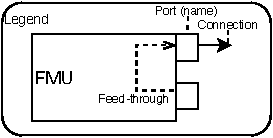
\includegraphics{images/FMU_legendpdf.pdf}
    \caption{FMU representation}
    \label{fig:fmu_legend}
\end{figure}

An FMU can visually be displayed as in Figure \ref{fig:fmu_legend} where a simple co-simulation scenario is shown.

\begin{definition}[Output Computation]\label{def:getout}
The $\fget{c}(\dontcare, \outputvar{c})$ represents the calculation of output $\outputvar{c}$ of $c \in \fmus$. Given a co-simulation state, it checks whether all inputs that feed-through to $\outputvar{c}$ are defined.
\end{definition}

\begin{definition}[Input Computation]\label{def:setin}
The $\fset{c}(\dontcare, \inputvar{c}, \inputV)$ represents the setting of input $\inputvar{c}$  of $c \in \fmus$. Given a co-simulation state, it checks whether all outputs connected to $\inputvar{c}$ are defined.
\end{definition}

\begin{definition}[Interconnected variable]
An interconnected variable v of a co-simulation scenario $\tuple{\fmus, \coupling}$ is defined as $v \in \allinputs \cup \alloutputs$, then $\coupling : \allinputs \to \alloutputs$.
\end{definition}

\subsection{INTO-CPS Maestro 2}\todo{We can have some more in this section - potentially half a page?}
INTO-CPS Maestro 2\footnote{currently in alpha \url{https://github.com/INTO-CPS-Association/maestro/tree/2.0.0-alpha}}\cite{thule_maestro2_2019} is an FMI-based co-simulation framework set to supersede Maestro\cite{Maestro}. The philosophy of the framework is to apply plugins to generate co-simulation specifications expressed in the domain specific language called Maestro Base Language (MaBL). Such specifications are then interpreted and executed resolving in the execution of a co-simulation.

\section{Generation of an Initialization Order}\label{sc:initilization}
FMI defines certain information about the initialization order described through different states of a co-simulation. The initialization phase covers the two states (in chronological order):
\begin{itemize}
    \item \textit{Instantiated}
    \item \textit{Initialization Mode}
\end{itemize}
In each of the two states, different groups of FMU variables can be assigned a value. The groups are defined by FMI based on predicates on the characteristics of the variables (\textit{causality}, \textit{initial} and \textit{variability}). These predicates have been extracted and used in the implementation. 
An example of a group is the \textit{INI}-group that consists of FMU variables with $initial = exact\, \lor initial = \,approx $  and $variability \neq constant$. All variables of this group should be set in the \textit{Instantiated}-phase of a co-simulation, and since they have no dependencies/connections to other FMU variables, the order is insignificant. However, all variables of each FMU are group together to perform the fewest possible operations in the initialization. The FMI specification does allow multiple variables of a single FMU to be set in parallel.

In the \textit{Initialization Mode} state, the variables of all FMUs should be defined if no circular dependencies exist. 
The variables with \textit{causality = parameter} of each FMU are set first, and the order of which they are set is again insignificant as they are independent.
Afterwards the interconnected variables should be defined, but as stated by the definitions \ref{def:feedthrough}, \ref{def:getout} and \ref{def:setin} the operations \textit{get} and \textit{set} \textbf{require} a specific initialization order. 

The correct initialization order of these interconnected variables has been calculated using the method described in Gomes et al. \cite{Gomes2019b}. The method is to use a topological ordering as the initialization order. The topological ordering is based on a graph of the interconnected FMU variables and internal connections. 
The calculation of an initialization order can be performed in linear based on the number of both external and internal connections. The calculation should also identify circular dependencies between the interconnected FMU variables since they would invalidate the co-simulation result. This paper's main contribution is to calculate an initialization order of a co-simulation and guarantee absence of cycles in a system being simulated.

\subsection{Structure of the graph}
The graph is constructed based on the interconnected variables and internal connections (feed-through). Each interconnected variable in the system represents a node, and the edges are based on these connections. The edges of this graph represent precedence constraints based on the algebraic dependencies of the interconnected variables. Please see definition \ref{def:initialization_graph} for a formal definition of the graph.

\begin{definition}[Initialization Graph]\label{def:initialization_graph}
  Given a co-simulation scenario $\tuple{\fmus, \coupling}$, and a set of feed-through dependencies $\bigcup_{c \in \fmus} \set{\feedthrough{c}}$, we define the Initialization Graph where each node represents a port $\outputvar{c} \in \outputs{c}$ or $\inputvar{c} \in \inputs{c}$ of some fmu $c \in \fmus$. The edges are created according to the following rules:
  \begin{compactenum}
    \item For each $c \in \fmus$ and $\inputvar{c} \in \inputs{c}$, if $\coupling(\inputvar{c}) = \outputvar{d}$, add an edge $\outputvar{d} -> \inputvar{c}$.
    \item For each $c \in \fmus$ and $(\inputvar{c},\outputvar{c}) \in \feedthrough{c}$, add an edge $\inputvar{c} -> \outputvar{c}$.
  \end{compactenum}
\end{definition}

\noindent As previously stated, a valid initialization order can only be calculated from an Initialization Graph if it does not contain any strongly connected components. This insight can be used to specify for which co-simulation scenarios a correct initialization order can be generated. A valid co-simulation scenario to calculate an initialization order from is defined in definition \ref{def:valid_graph}.

\begin{definition}[Validity criteria for Generation of an Initialization Graph]\label{def:valid_graph}
  The Initialization Graph is valid if the given a co-simulation scenario $\tuple{\fmus, \coupling}$, and a set of feed-through dependencies $\bigcup_{c \in \fmus} \set{\feedthrough{c}}$.
  $\forall c \in \fmus \implies \nexists \inputvar{} \in \inputs{c}, \outputvar{} \in \outputs{c}: (\inputvar{},\outputvar{}) \in \feedthrough{c} \land Path(\outputvar{}, \inputvar{})$\\
  Where Paths is defined as the transitive closure of $Path = L \cup \bigcup_{c \in \fmus} \set{\feedthrough{c}}$
\end{definition}

All co-simulation scenarios satisfying definition \ref{def:valid_graph} is guaranteed to have a valid initialization order.  

\subsection{Three Tank Example}
The structure of the Initialization Graph will be described using a small example. 
The example is based on three water tanks that are filled and emptied. The first tank is filled from a source with a valve that may be turned on and off. The outflow of the first tank constitutes the inflow of the second, and so forth. A discrete-event controller monitors the level of the third tank and controls a valve to a drain. When the water level of the tank reaches a particular level (defined in the controller), the controller sends a command to the tank to empty using an exit valve. An illustration of the three water tanks can be seen in Figure \ref{fig:watertank}. A diagram of the FMUs showing the interconnections of the FMU variables in the system can be in Figure \ref{fig:watertank}. It should be noted that all internal connections that do not \textit{feed-through} have been omitted to simplify the diagram since they do not influence the initialization order and are not included in the graph defined in definition \ref{def:initialization_graph}. 

\begin{figure}[H]
    \begin{minipage}{0.40\textwidth}
    \centering
        \centering
    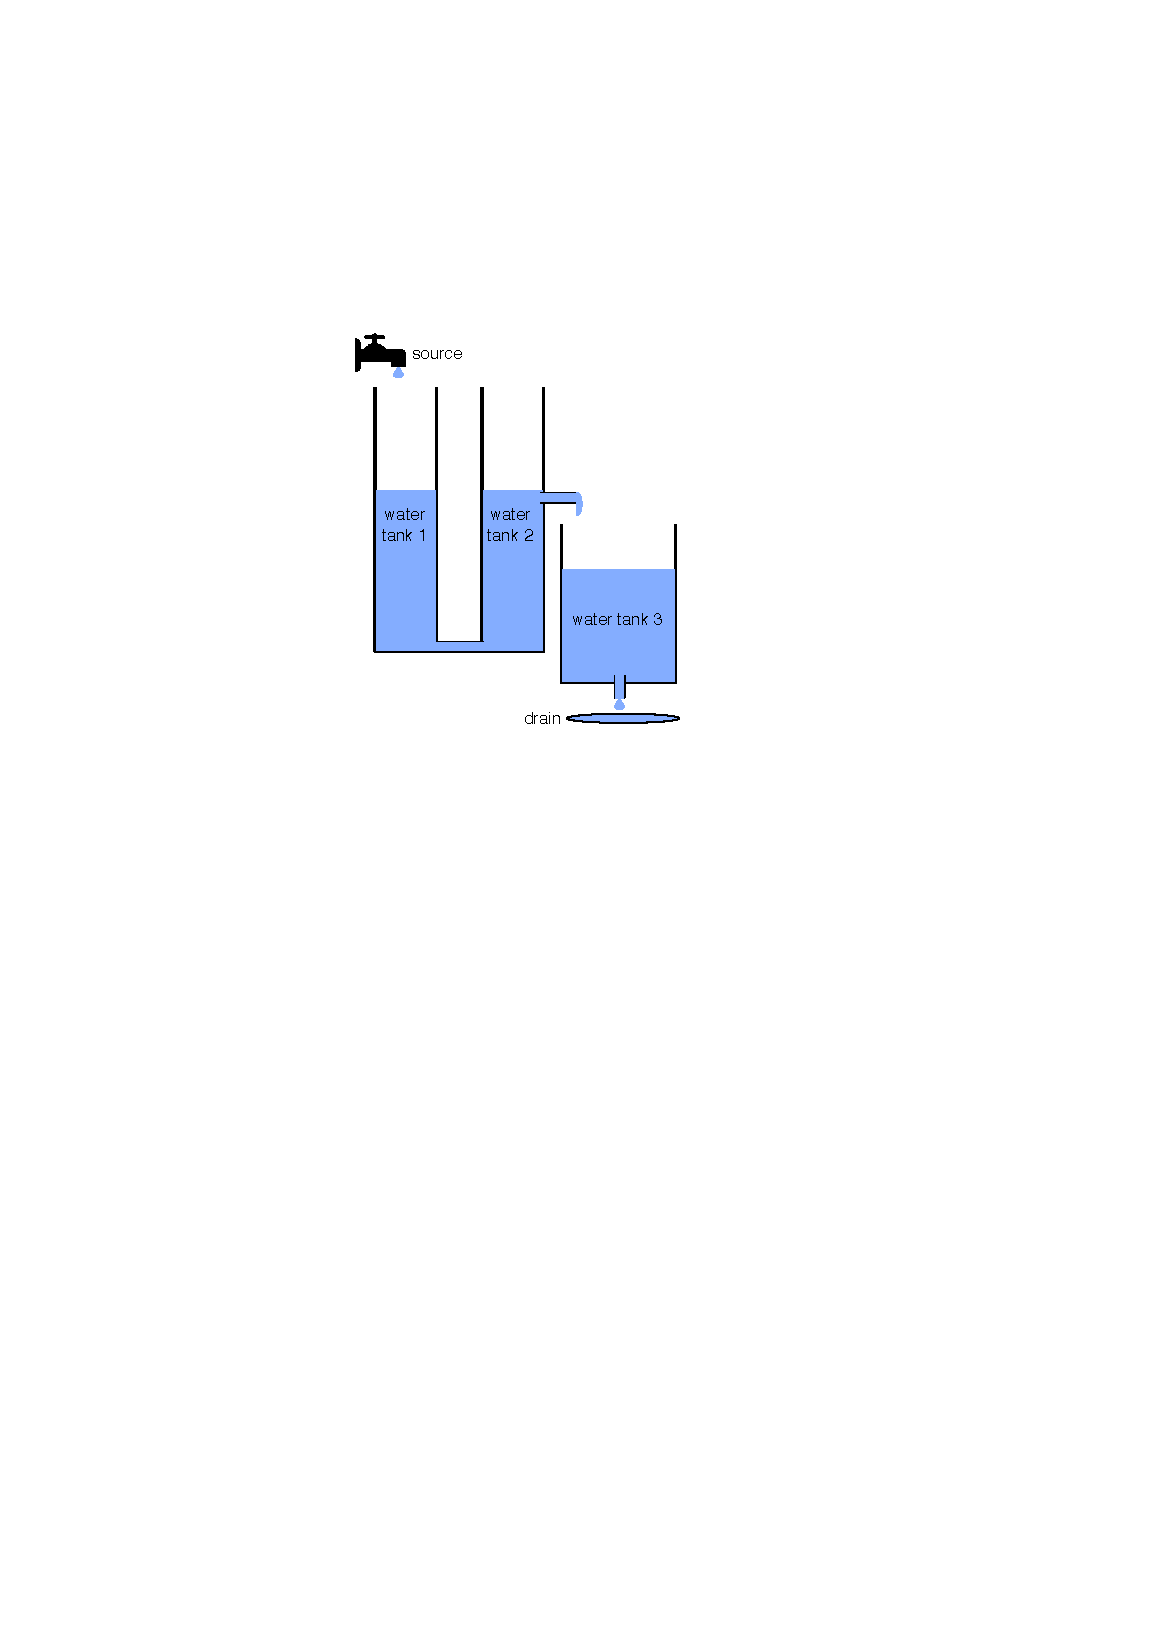
\includegraphics[width=1\textwidth]{images/ttwt_overview.pdf}
    \end{minipage}
    \begin{minipage}{0.60\textwidth}
        \centering
    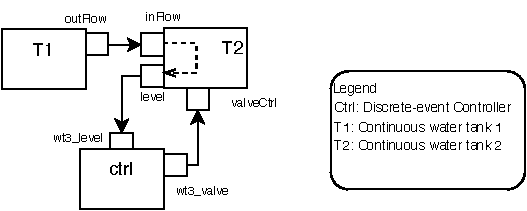
\includegraphics[width=1\textwidth]{images/threetank_FMU.pdf}
    \end{minipage}
    \caption{Three tank case study}
    \label{fig:watertank}
\end{figure}

\noindent A correct initialization order can be calculated since there are no circular dependencies in the system, the Initialization Graph is valid based on definition \ref{def:valid_graph}. The corresponding Initialization Graph of the three tank system can be seen in figure \ref{fig:initilizationGraph}. As it can be seen from the Initialization Graph, it is a disconnected graph meaning there are no limitations on the order of the initialization between the two sub-graphs. Nevertheless, in this case, an optimization of the initialization order can be made, using the fact that the FMI specification allows the set/get variables of the same FMU to be performed in bulk. This optimization can be made by setting the two inputs of \textit{T2} simultaneously (by the same operation). The definition of the optimization can be found in definition \ref{def:optimization}.
It is not challenging to calculate the initialization order in this simple example. However, knowledge about the internal connections of each FMU is needed in order to calculate the initialization order due to \textit{feed-through} in FMU \textit{T2}. The strategy for calculating the initialization order scales to more advanced systems with an arbitrary number of FMUs and interconnected variables. Furthermore, an initialization order can be found as long a the Initialization Graph satisfies the criteria of definition \ref{def:valid_graph}.

\begin{figure}
    \centering
      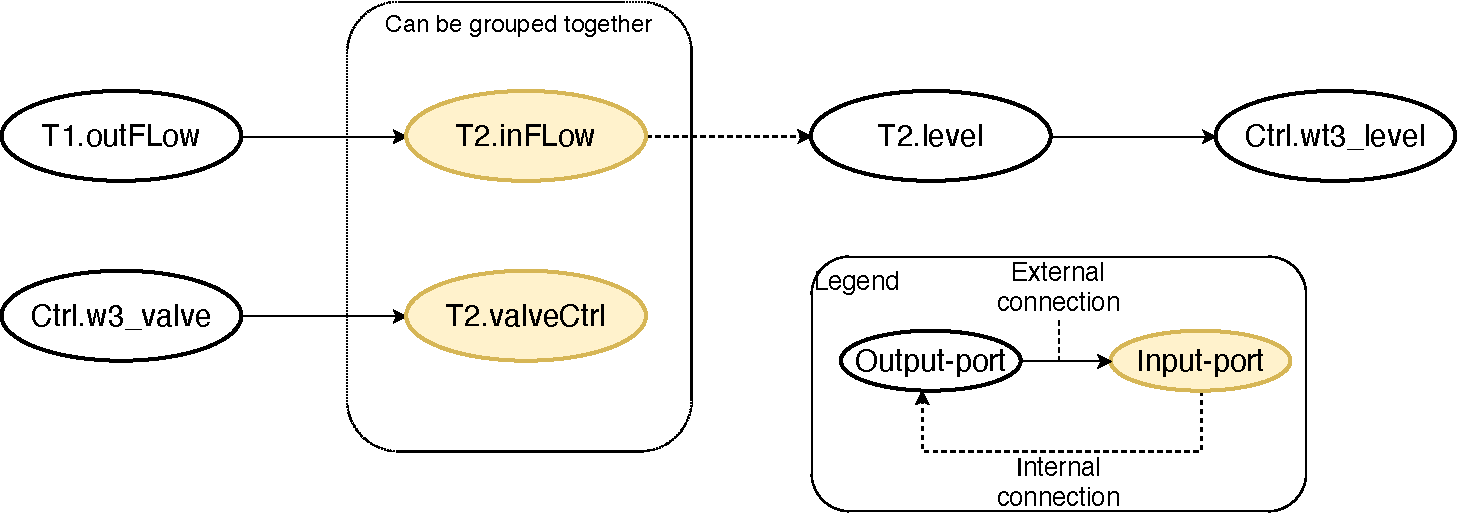
\includegraphics[width=0.95\textwidth]{images/threetank_initialization.pdf}
    \caption{Initialization Graph of three tank}
  \label{fig:initilizationGraph}
\end{figure}


\begin{definition}[Optimization of a Initialization procedure]\label{def:optimization}
  Given an initialization procedure $\sequence{\initcall_i}_{i \in \setnat}$ with a finite ordered sequence of FMU function calls $\functioncall_i \in \allfunctioncalls = \bigcup_{c \in \fmus} \set{\fset{c},\fget{c}},$ and $i$ denoting the order of the function call. It can be optimized if $\exists \functioncall_i, \functioncall_{i +1} \in \allfunctioncalls : \exists c \in \fmus :(\functioncall_i \in {\fset{c}} \land \functioncall_{i+1} \in {\fset{c}}) \lor (\functioncall_i \in {\fget{c}} \land \functioncall_{i+1} \in {\fget{c}})$
\end{definition}
This optimization uses the fact that the FMI specification allows to \textit{set} or \textit{get} variables of the same FMU to be performed in bulk by grouping interconnected variables of the same FMU with others with similar characteristic.
Since an Initialization procedure is defined in the same they as other co-simulation steps. The optimization process described in definition \ref{def:optimization} is valid for an arbitrary co-simulation step. The only difference between an arbitrary co-simulation step and an initialization procedure is the size of the graph on which the topological sorting is performed. 
The correctness of this optimization can be established by the proof of using the Initialization Graph's topological ordering as the initialization order described by Gomes et al. This proof is still valid since this optimization does not change the structure of the Initialization Graph. 
This optimization strategy potentially will not find all valid optimizations of a co-simulation scenario since it works on a co-simulation step (a topological order of a graph), which is not necessarily unique for a given co-simulation scenario/graph. To perform all possible optimizations of a co-simulation step, a more advanced optimization strategy should be used, or the optimization should be performed on the set of all valid co-simulation steps.

\section{Realization of a Maestro 2 Plugin}\label{sc:implementation}
This approach has been realized as a Maestro 2 plugin that generates the \textit{Initialization}-phase of a co-simulation specification expressed in MaBL. It calculates the specification based on a list of FMU-components, the simulation scenario as defined in definition \ref{def:cosim_scenario}, and a specific plugin-configuration to let the user supply initial values of FMU variables with $causality=parameter$. The plugin optimizes the initialization order of the initialization by grouping operations that can be executed in \textit{parallel} to take advantage of FMI's ability to set or get multiple variables in bulk from the same FMU. The criteria for this optimization is defined in definition \ref{def:optimization}. 
The developed plugin has been tested on numerous co-simulation examples from the INTO-CPS universe\todo{should I add a footnote} and compared with the existing \textit{Initializer} of Maestro. The plugin has been tested in the whole Maestro 2 pipeline to practically verify that it can be used in a co-simulation where the generated initialization procedure is integrated as a part of a complete co-simulation to verify the initialization procedure's integration with a master algorithm.

\subsection{Topological sorting}
The algorithm for calculating the topological order of the Initialization Graph defined in definition \ref{def:initialization_graph} is Tarjan's algorithm\cite{tarjan_1972}. The algorithm was selected since it solves two of the central issues of the initialization-phase of the co-simulation.
\begin{itemize}
    \item Identifies circular dependencies between interconnected variables (strongly connected components)
    \item Performs a topological sorting of the Initialization Graph
\end{itemize}
The algorithm is furthermore well-established, and there exist formal proofs of its correctness and properties\cite{stefan_merz}. 

The topological sorting algorithm was implemented in Scala. The choice of Scala is motivated by the relation to JVM and the connection to Slang and the Logika framework\cite{inbook}. The connection to Slang and Logika will be used in the future work of formally verifying the plugin and explore how the contract-based nature of Slang can be used to obtain more trustworthy results of co-simulations.

\subsection{Verification of the approach}
The plugin and the approach behind it have been verified in several different ways. Gomes et al. have in \cite{gomes_lucio_vangheluwe_2019} proved the correctness of using the topological order of a similar graph to generate not only the initialization order but also the order for a co-simulation master-algorithm. The purpose of the publication by Gomes et al. is a little different from the one of this paper. Gomes et al. are interested in both generating an initialization and master-algorithm, meaning they also need to focus on the time of each FMU. They also define their graph using methods (Set, Get, doStep) instead of interconnected variables, which is the approach described in this paper. This simplification is valid since this approach only cares about initialization and, therefore, does not need to care about the time of each FMU. This does that we can omit all the $doStep$ nodes and all edges connected to them from the graph by Gomes et al., this approach does, therefore, end up with a subgraph of the graph by Gomes et al. The proof from \cite{gomes_lucio_vangheluwe_2019} can therefore trivial be modified to the graph/approach presented in this paper.

The main contribution of Gomes et al. is an implementation of the FMI specification in Prolog freely available to be used in other projects. The Prolog implementation was used in their research to verify their proposed approach for generation of co-simulation algorithms. The realization encapsulates all the rules of a valid master-algorithm and an initialization algorithm. As a part of this work, integration from the plugin has been created to the Prolog realization. This integration has been realized in order to verify the correctness of the calculated initialization order against an established and recognized method. The integration is based on JIProlog\cite{}, and it is querying the Prolog database with a co-simulation environment and an initialization order. The integration requires substantially mapping of the objects between the Java code of Maestro 2 and the Prolog implementation, and due to the described differences between the two graphs a mapping from the graph of ports to the graph of operations is needed. This mapping is based on the definitions \ref{def:getout} and \ref{def:setin}.

The Prolog code can generate an initialization order, but this functionality haven't been used for several reasons. The main reason for not generating the initialization order using the Prolog code is based on performance considerations, and the approach taken in this paper does also ensure absence of circular dependencies between the interconnected FMU variables. 

\section{Related Work}
Gomes et al. \cite{Gomes2019} propose a strategy for the generation of co-simulation algorithms for FMI-based scenarios based on a graph of the operations of a co-simulation step. However, there are some key differences between their work and ours since the method they purpose does not handle algebraic loops. Furthermore, the approach taken in this paper is only concerned with the initialization procedure of a co-simulation.

The requirement of freedom of algebraic loops of FMI-based co-simulation scenarios to obtain a deterministic composition result of a co-simulation master algorithm was required by Broman et al. \cite{BromanCompositionCo-Simulation}. They proposed to use the topological sorting of a dependency graph of the interconnected variables to detect algebraic loops and discover the partial order of a co-simulation step. This insight 

Prior work by Amalio et al. \cite{Amalio2016CheckingCo-simulation} has been investigating how to ensure the absence of algebraic loops in FMU based co-simulation scenarios by statically checking the SysML CPS architectural design. The publication's purpose is partly very similar to ours - to guarantee the absence of algebraic loops in a co-simulation scenario. Nevertheless, their approach is only concerned with ensuring the absence of algebraic-loops since their approach is analyzing an architecture design; the calculation of the initialization order is of no interest.

\section{Concluding remarks}\label{sc:summary}
This work uses a topological ordering of a dependency graph of the interconnected FMUs variable and internal FMU variable connections along with predicates from the FMI specification to calculate a correct initialization order for a co-simulation scenario. The plugin optimizes the calculated initialization order by grouping variables with similar characteristics to perform the fewest possible operations in the initialization procedure.
This approach supports the initialization of a co-simulation scenario containing algebraic loops by utilization of fixed point iteration. The approach discards all co-simulation scenarios, not adhering to the law of convergence \ref{def:convergence}.
It is possible to combine the approach with an arbitrary master algorithm to run a co-simulation. \\
The approach is realized as a plugin for the open-source INTO-CPS Maestro 2 tool and verified against the existing \textit{Initializer} and the calculated initialization order was verified against an established co-simulation Algorithm Generator and Verifier implemented in Prolog\cite{gomes_lucio_vangheluwe_2019}\\
Future work includes formal verification of the plugin using the Logika framework\cite{inbook}.
We will also look into the generation of a verification strategy for the whole Maestro 2 framework to examine how different forms of verification jointly can extend the trust of the correctness of the result of a co-simulation. 

\paragraph*{\textbf{Acknowlegements.}}We would like to thank Stefan Hallerstede, Christian Møldrup Legaard, and Peter Gorm Larsen for providing valuable input to this paper and the developed plugin.
%
% ---- Bibliography ---

\bibliographystyle{splncs04}
\bibliography{gen_bib}


\end{document}
